\documentclass[aspectratio=169,10pt]{beamer}

\usetheme{Madrid}
\usecolortheme{seahorse}

\usepackage{amsmath,amssymb,amsfonts}
\usepackage{mathtools}
\usepackage{listings}
\usepackage{xcolor}
\usepackage{graphicx}

\graphicspath{{figures/}}

% Code style
\lstset{
    basicstyle=\ttfamily\scriptsize,
    commentstyle=\color{green!50!black}\itshape,
    keywordstyle=\color{blue}\bfseries,
    stringstyle=\color{red},
    breaklines=true,
    numbers=left,
    numberstyle=\tiny\color{gray},
    frame=single,
    backgroundcolor=\color{white}
}

% Math operators
\newcommand{\R}{\mathbb{R}}
\newcommand{Hilb}{H}
\newcommand{\E}{\mathbb{E}}
\newcommand{K}{K}
\newcommand{\N}{\mathbb{N}}
\newcommand{\zo}{\{0\}}
\newcommand{\dom}{\mathrm{dom}}
\newcommand{\epi}{\mathrm{epi}}
\newcommand{\ri}{\mathrm{ri}}
\newcommand{\cont}{\mathrm{cont}}
\newcommand{\gra}{\mathrm{gra}}
\newcommand{\Argmin}{\mathrm{Argmin}}
\newcommand{\Prox}{\mathrm{prox}}
\newcommand{\zer}{\mathrm{zer}}
\newcommand{\ran}{\mathrm{ran}}
\newcommand{\id}{\mathrm{id}}
\newcommand{\sign}{\mathrm{sign}}
\newcommand{\sri}{\mathrm{sri}}
\newcommand{\bdry}{\mathrm{bdry}}
\newcommand{\cl}{\mathrm{cl}}
\newcommand{\conv}{\mathrm{conv}}
\newcommand{\cone}{\mathrm{cone}}
\newcommand{\lin}{\mathrm{lin}}
\newcommand{\aff}{\mathrm{aff}}
\newcommand{\ridom}[1]{\ri(#1 \cap \mathrm{dom}\,f)}

\setbeamertemplate{footline}[frame number]

\title[Chapter 16: Subdifferentiability]{Chapter 16: Subdifferentiability of Convex Functions}
\subtitle{Convex Analysis and Monotone Operator Theory in Hilbert Spaces}
\author{Based on Bauschke \& Combettes (2017)}
\date{}

\begin{document}

\frame{\titlepage}

\begin{frame}
\frametitle{Chapter Overview}
\begin{itemize}
  \item \textbf{16.1:} Basic properties of subdifferentials
  \item \textbf{16.2:} Convex functions and subdifferentials
  \item \textbf{16.3:} Lower semicontinuous convex functions
  \item \textbf{16.4:} Subdifferential calculus (chain rule, sum rule, composition)
  \item \textbf{16.5:} Subdifferential of composition and coderivatives
\end{itemize}

\vspace{1cm}

\textbf{Key Concepts:}
\begin{itemize}
  \item Subgradients and supporting hyperplanes
  \item Fermat's rule and optimality
  \item Proximal operators and monotonicity
  \item Calculus rules for subdifferentials
\end{itemize}
\end{frame}

% =====================================================================
% SECTION: INTRODUCTION AND BASICS
% =====================================================================

\section{Basic Concepts}

\begin{frame}
\frametitle{Subgradients: Definition and Geometry}

\textbf{Definition 16.1:} Let $f : H \to \overline{\R}$ be proper. A vector $u \in H$ is a \textbf{subgradient} of $f$ at $x \in \mathrm{dom}\,f$ if:

\[
(\forall y \in H) \quad \langle y - x \mid u \rangle + f(x) \le f(y)
\]

The \textbf{subdifferential} $\partial f(x)$ is the set of all subgradients:

\[
\partial f(x) = \{u \in H \mid (\forall y \in H) \, \langle y - x \mid u \rangle + f(x) \le f(y)\}
\]

\vspace{0.5cm}

\textbf{Geometric Interpretation:} $u$ is the ``slope'' of a supporting hyperplane to the epigraph of $f$ that touches the graph at $(x, f(x))$.

\begin{center}
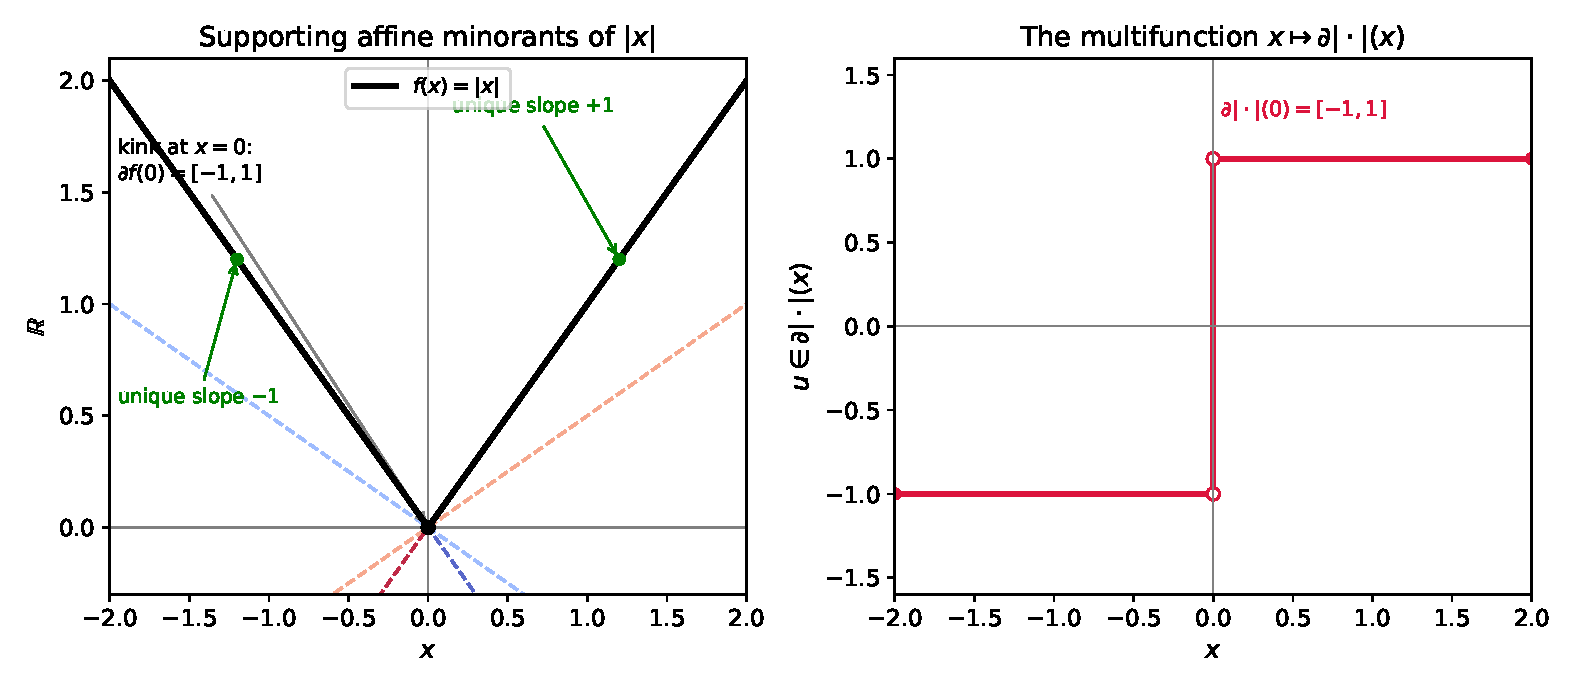
\includegraphics[width=0.5\textwidth]{fig_abs_subdifferential.pdf}
\end{center}
\end{frame}

\begin{frame}
\frametitle{Fermat's Rule: First-Order Optimality}

\textbf{Theorem 16.3 (Fermat's Rule):} Let $f : H \to \overline{\R}$ be proper. Then:

\[
\Argmin f = \zer \partial f = \{x \in H \mid 0 \in \partial f(x)\}
\]

\vspace{0.5cm}

\textbf{Proof Sketch:}
\begin{itemize}
  \item $x \in \Argmin f \Leftrightarrow (\forall y \in H) \, \langle y - x \mid 0 \rangle + f(x) \le f(y)$
  \item This is equivalent to $0 \in \partial f(x)$
\end{itemize}

\vspace{0.5cm}

\textbf{Key Consequence:} Finding a minimizer is equivalent to finding a point where $0$ is a subgradient!

\begin{center}
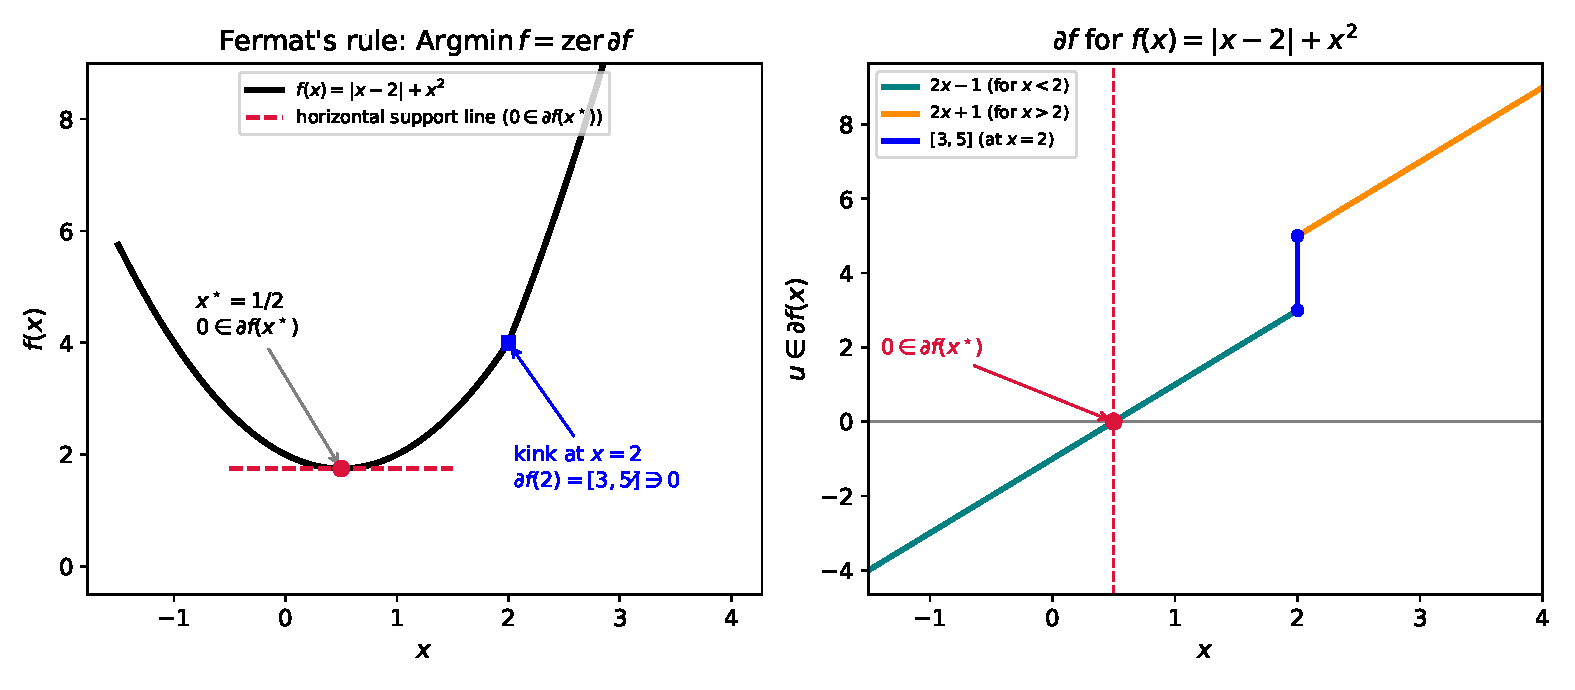
\includegraphics[width=0.55\textwidth]{fig_fermat_rule.pdf}
\end{center}
\end{frame}

\begin{frame}[fragile]
\frametitle{Example: Computing Subdifferentials}

\textbf{Example 16.12:} For $f(x) = \frac{1}{2}\|x\|^2$, we have $\partial f = \mathrm{Id}$ (the identity operator).

\vspace{0.5cm}

\textbf{Example 16.15:} For $f(\xi) = |\xi|$ in $\R$:

\[
\partial |\xi| = \begin{cases}
  \{-1\}, & \text{if } \xi < 0 \\
  [-1, 1], & \text{if } \xi = 0 \\
  \{1\}, & \text{if } \xi > 0
\end{cases}
\]

\vspace{0.5cm}

\textbf{Example 16.32:} For the norm $f(x) = \|x\|$:

\[
\partial \|x\| = \begin{cases}
  \left\{\frac{x}{\|x\|}\right\}, & \text{if } x \ne 0 \\
  B(0; 1), & \text{if } x = 0
\end{cases}
\]

\begin{center}
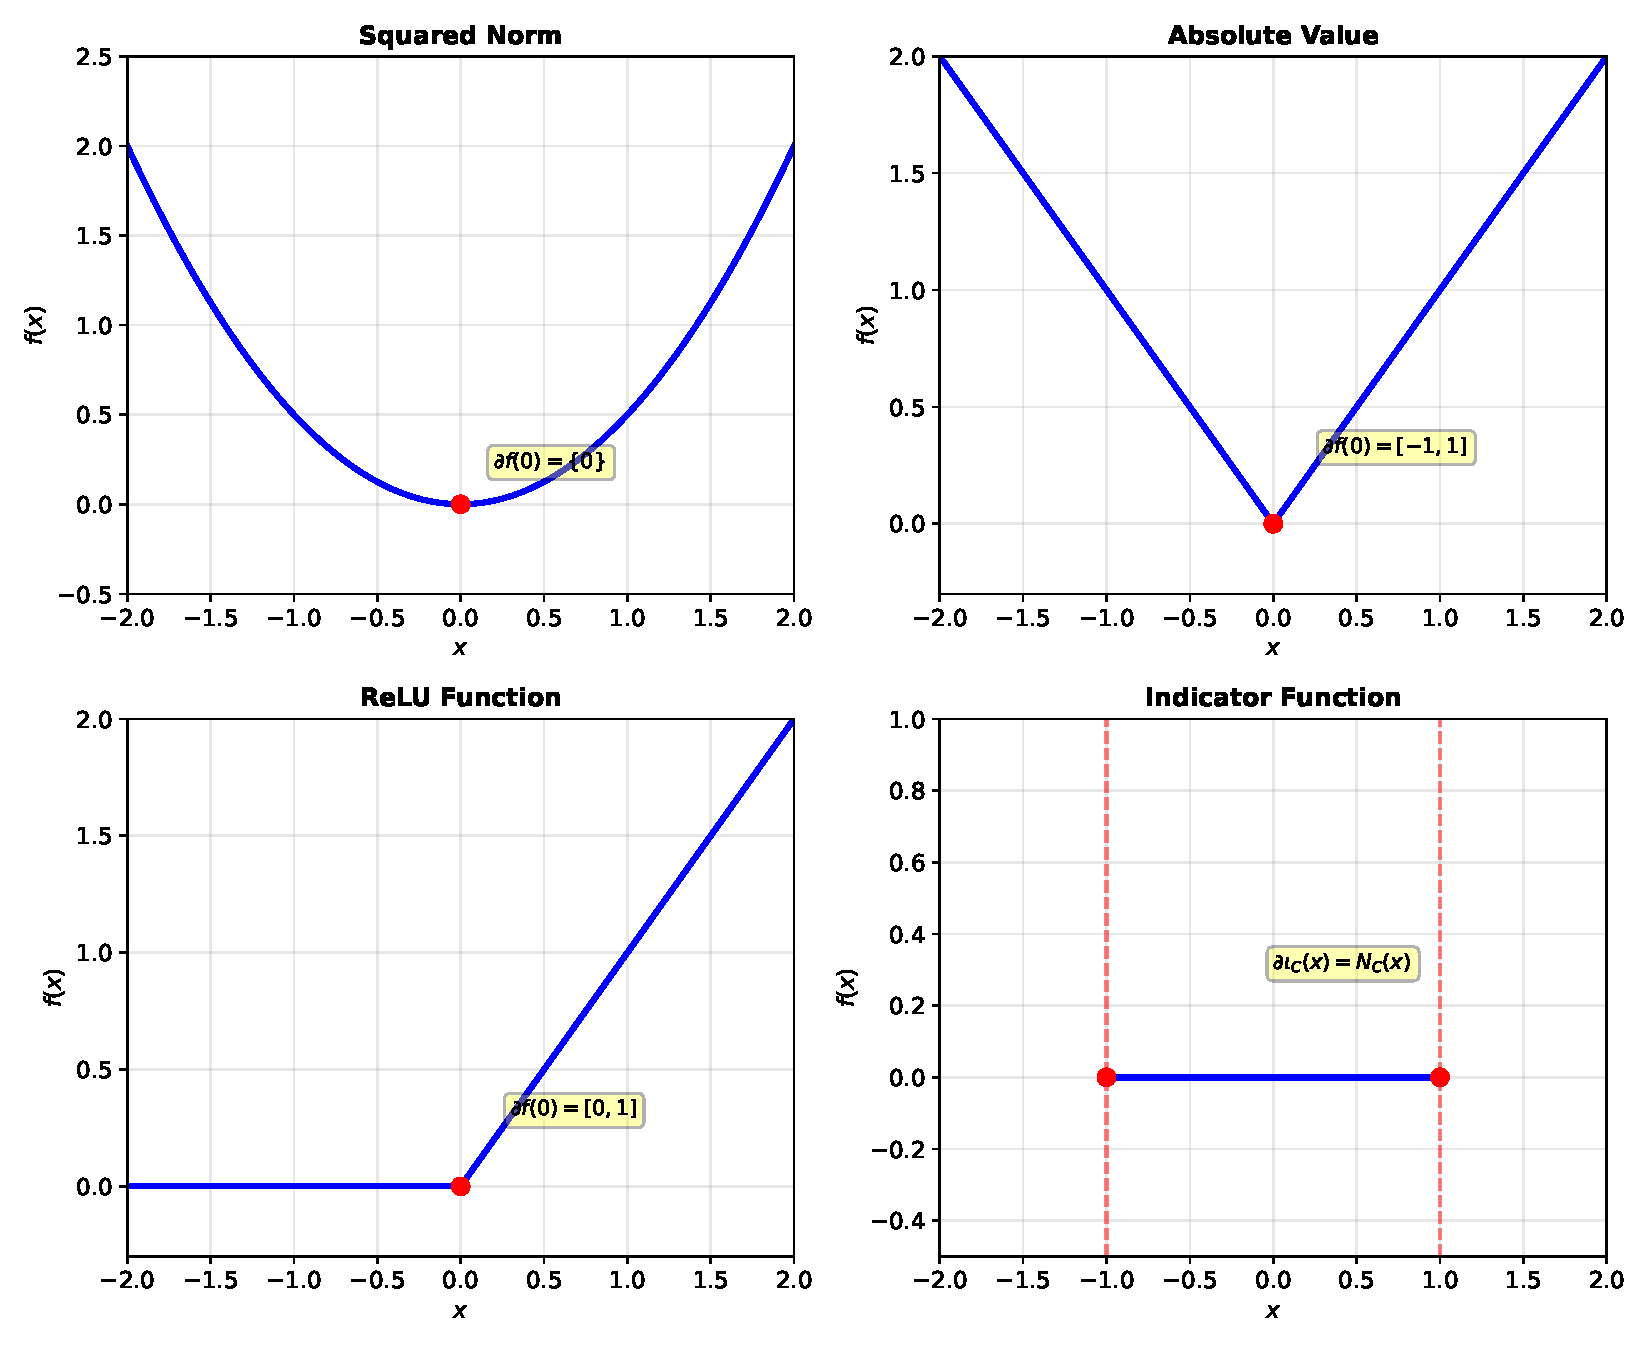
\includegraphics[width=0.6\textwidth]{fig_subdiff_examples.pdf}
\end{center}
\end{frame}

% =====================================================================
% SECTION: BASIC PROPERTIES
% =====================================================================

\section{Basic Properties}

\begin{frame}[allowframebreaks]
\frametitle{Basic Properties of Subdifferentials}

\textbf{Proposition 16.4:} Let $f : H \to \overline{\R}$ be proper and $x \in \dom f$. Then:

\begin{itemize}
  \item[(i)] $\dom \partial f \subseteq \dom f$
  \item[(ii)] $\partial f(x) = \bigcap_{y \in \dom f} \{u \in H \mid \langle y - x \mid u \rangle \le f(y) - f(x)\}$
  \item[(iii)] $\partial f(x)$ is closed and convex
  \item[(iv)] If $x \in \dom \partial f$, then $f$ is lower semicontinuous and weakly lower semicontinuous at $x$
\end{itemize}

\vspace{0.5cm}

\textbf{Proposition 16.5 (Connection to Conjugate):} Let $f : H \to \overline{\R}$ be proper. Then:
\[
f^{**}(x) = f(x) \quad \text{and} \quad \partial f^{**}(x) = \partial f(x)
\]

\framebreak

\textbf{Proposition 16.6 (Scaling and Composition):} Let $\lambda \in \R_{++}$, $L \in \mathcal{B}(H, K)$, and $g : K \to \overline{\R}$ proper. Then:

\begin{itemize}
  \item[(i)] $\partial(\lambda f) = \lambda \partial f$
  \item[(ii)] If $\dom(g \circ L) \cap \dom f \ne \emptyset$, then $\partial(f + g \circ L) = \partial f + L^* \circ (\partial g) \circ L$
\end{itemize}

\framebreak

\textbf{Proposition 16.7 (Subdifferential on Product Spaces):}

Let $H = \bigoplus_{i \in I} H_i$ and $f : H \to \overline{\R}$ proper. For $\mathbf{x} = (x_i)_{i \in I}$:

\[
\partial f(\mathbf{x}) \subseteq \times_{i \in I} \partial(f \circ R_i)(x_i)
\]

where $R_i : H_i \to H$ is the natural embedding.

\end{frame}

% =====================================================================
% SECTION: CONVEX FUNCTIONS
% =====================================================================

\section{Convex Functions}

\begin{frame}
\frametitle{Subdifferentials of Convex Functions}

\textbf{Remark 16.2:} For $f \in \Gamma_0(H)$, we have $\dom \partial f \ne \emptyset$ (Theorem 9.20 + Corollary 16.39).

\vspace{0.5cm}

\textbf{Proposition 16.16:} Let $f : H \to \overline{\R}$ be proper and convex. Then:
\[
u \in \partial f(x) \Leftrightarrow (u, -1) \in N_{\mathrm{epi}\,f}(x, f(x)) \Leftrightarrow f(x) + f^*(u) = \langle x \mid u \rangle
\]

This last equality is the \textbf{Fenchel-Young equality}.

\vspace{0.5cm}

\textbf{Proposition 16.17:} Let $f : H \to \overline{\R}$ be proper and convex, $x \in \dom f$. Then:

\begin{itemize}
  \item[(i)] If $\mathrm{int}(\dom f) \ne \emptyset$ and $x \in \bdry(\dom f)$, then $\partial f(x)$ is empty or unbounded
  \item[(ii)] If $x \in \mathrm{cont} f$, then $\partial f(x)$ is nonempty and weakly compact
  \item[(iii)] If $x \in \mathrm{cont} f$, then $\exists \rho \in \R_{++}$ such that $\partial f(B(x; \rho))$ is bounded
  \item[(iv)] If $\mathrm{int}(\dom f) \ne \emptyset$, then $\mathrm{int}(\dom f) \subseteq \dom \partial f$
\end{itemize}
\end{frame}

\begin{frame}
\frametitle{Finite-Dimensional Results}

\textbf{Corollary 16.18:} When $H$ is finite-dimensional and $f : H \to \overline{\R}$ is proper and convex:

\begin{itemize}
  \item[(i)] $\emptyset \ne \ri(\dom f) \subseteq \dom \partial f$
  \item[(ii)] $f$ possesses a continuous affine minorant
\end{itemize}

\vspace{0.5cm}

\textbf{Corollary 16.21:} In finite dimensions, for $f \in \Gamma_0(H)$, the following are equivalent:

\begin{itemize}
  \item $f$ is supercoercive
  \item $(\forall u \in H) \, f(\langle \cdot \mid u \rangle)$ is coercive
  \item $\dom f^* = H$
\end{itemize}

\vspace{0.5cm}

\begin{center}
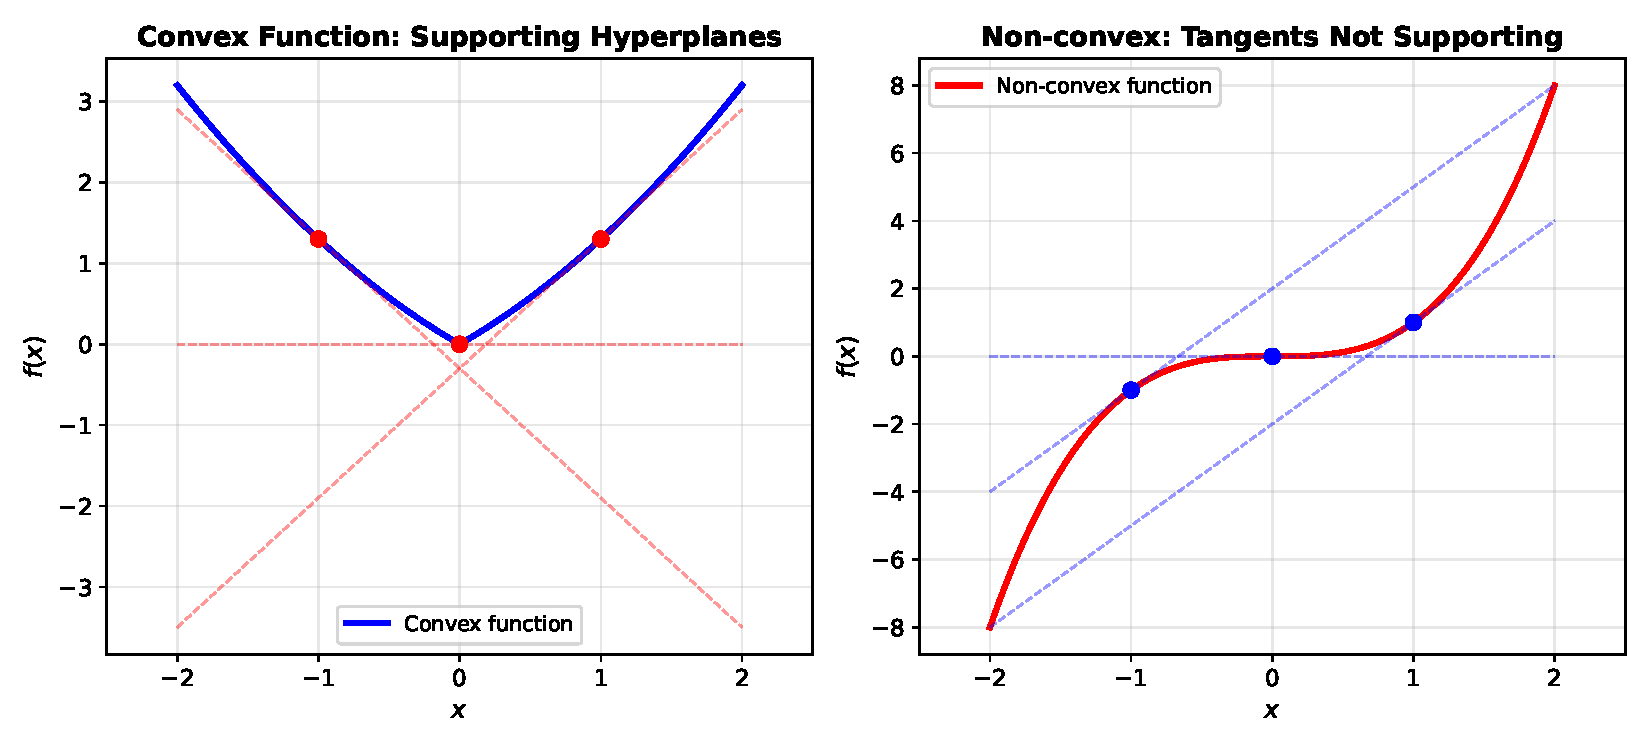
\includegraphics[width=0.6\textwidth]{fig_convexity.pdf}
\end{center}
\end{frame}

% =====================================================================
% SECTION: LOWER SEMICONTINUOUS FUNCTIONS
% =====================================================================

\section{Lower Semicontinuous Convex Functions}

\begin{frame}[allowframebreaks]
\frametitle{Lower Semicontinuous Convex Functions}

\textbf{Definition:} A function $f : H \to \overline{\R}$ is in $\Gamma_0(H)$ if it is proper, convex, and lower semicontinuous.

\vspace{0.5cm}

\textbf{Proposition 16.24:} If $f \in \Gamma_0(H)$ is positively homogeneous, then $f = \sigma_C$ where $C = \partial f(0)$.

\vspace{0.5cm}

\textbf{Proposition 16.25:} If $f \in \Gamma_0(H)$ with $\mathrm{int}(\dom f) \ne \emptyset$, then:
\[
f = (f + \iota_{\mathrm{int}(\dom f)})^{**}
\]

\framebreak

\textbf{Proposition 16.27:} For $f \in \Gamma_0(H)$:
\[
\mathrm{int}(\dom f) = \mathrm{cont} f \subseteq \dom \partial f \subseteq \dom f
\]

\vspace{0.5cm}

\textbf{Remark 16.28:} The set $\dom \partial f$ may not be convex! Example: $f(\xi_1, \xi_2) = \max\{g(\xi_1), |\xi_2|\}$ in $\R^2$.

\framebreak

\textbf{Theorem 16.29 (Characterizations):} For $f \in \Gamma_0(H)$, $x \in H$, $u \in H$, the following are equivalent:

\begin{itemize}
  \item[(i)] $(x, u) \in \gra \partial f$
  \item[(ii)] $(u, -1) \in N_{\mathrm{epi}\,f}(x, f(x))$
  \item[(iii)] $f(x) + f^*(u) = \langle x \mid u \rangle$
  \item[(iv)] $(u, x) \in \gra \partial f^*$
\end{itemize}

\vspace{0.5cm}

\textbf{Corollary 16.30:} For $f \in \Gamma_0(H)$:
\[
(\partial f)^{-1} = \partial f^*
\]

\end{frame}

% =====================================================================
% SECTION: SUBDIFFERENTIAL CALCULUS
% =====================================================================

\section{Subdifferential Calculus}

\begin{frame}[allowframebreaks]
\frametitle{Chain Rule for Subdifferentials}

\textbf{Proposition 16.42 (General Chain Rule):} Let $L \in \mathcal{B}(H, K)$, $f \in \Gamma_0(H)$, $g \in \Gamma_0(K)$, with $L(\dom f) \cap \dom g \ne \emptyset$. If $(f + g \circ L)^* = f^* \boxplus (L^* \circ g^*)$, then:

\[
\partial(f + g \circ L) = \partial f + L^* \circ (\partial g) \circ L
\]

\framebreak

\textbf{Example 16.43:} Let $f \in \Gamma_0(H)$ and $\gamma \in \R_{++}$. Then:
\[
\partial(f + (\gamma/2)\|\cdot\|^2) = \partial f + \gamma \cdot \mathrm{Id}
\]

\vspace{0.5cm}

\textbf{Proposition 16.44 (Proximal Operator):} For $f \in \Gamma_0(H)$ and $x, p \in H$:

\[
p = \Prox_f x \Leftrightarrow x - p \in \partial f(p)
\]

Equivalently:
\[
\Prox_f = (\mathrm{Id} + \partial f)^{-1}
\]

\vspace{0.5cm}

\textbf{Proposition 16.45:} For $f \in \Gamma_0(H)$:
\[
\ran(\mathrm{Id} + \partial f) = H
\]

This means the proximal operator is everywhere defined and single-valued.

\framebreak

\textbf{Remark 16.46 (Sum Rule Exactness):} Let $f, g \in \Gamma_0(H)$ with $\dom f \cap \dom g \ne \emptyset$. Then:

\[
f^* \boxplus g^* \text{ is exact on } \mathrm{dom}(f+g)^* \Rightarrow \partial(f+g) = \partial f + \partial g
\]

Conversely:
\[
\partial(f+g) = \partial f + \partial g \Rightarrow f^* \boxplus g^* \text{ is exact on } \mathrm{dom}(f+g)^*
\]

But the implication $\partial(f+g) = \partial f + \partial g \Rightarrow (f+g)^* = f^* \boxplus g^*$ can fail!

\end{frame}

\begin{frame}[allowframebreaks]
\frametitle{Subdifferential of Sum}

\textbf{Theorem 16.47 (Sum Rule):} Let $K$ be a Hilbert space, $f \in \Gamma_0(H)$, $g \in \Gamma_0(K)$, $L \in \mathcal{B}(H, K)$.

If one of these holds:
\begin{itemize}
  \item[(i)] $0 \in \sri(\dom g - L(\dom f))$
  \item[(ii)] $K$ finite-dimensional, $g$ polyhedral, $\dom g \cap L(\dom f) \ne \emptyset$
  \item[(iii)] $H, K$ finite-dimensional, $f, g$ polyhedral, $\dom g \cap L(\dom f) \ne \emptyset$
\end{itemize}

Then: $\partial(f + g \circ L) = \partial f + L^* \circ (\partial g) \circ L$

\framebreak

\textbf{Corollary 16.48 (Simple Cases):} For $f, g \in \Gamma_0(H)$, if one holds:

\begin{itemize}
  \item[(i)] $0 \in \sri(\dom f - \dom g)$
  \item[(ii)] $\dom f \cap \mathrm{int}(\dom g) \ne \emptyset$
  \item[(iii)] $\dom g = H$
  \item[(iv)] $H$ finite-dimensional and $\ri(\dom f) \cap \ri(\dom g) \ne \emptyset$
\end{itemize}

Then: $\partial(f + g) = \partial f + \partial g$

\framebreak

\textbf{Corollary 16.50 (Multiple Functions):} For $m \ge 2$ functions $f_i \in \Gamma_0(H)$, if one condition holds, then:

\[
\partial\left(\sum_{i \in I} f_i\right) = \sum_{i \in I} \partial f_i
\]

\vspace{0.5cm}

\textbf{Example 16.51:} The conditions are necessary! Example in $\R^2$ where $\partial(\iota_C + \iota_D) \ne \partial \iota_C + \partial \iota_D$ when $C \cap D = \{(0,0)\}$ only.

\end{frame}

\begin{frame}[allowframebreaks]
\frametitle{Mean Value Theorem}

\textbf{Theorem 16.56 (Mean Value):} Let $f \in \Gamma_0(H)$, $x_0, x_1 \in \dom f$. Suppose one holds:

\begin{itemize}
  \item[(i)] $0 \in \sri(\dom f - \mathrm{aff}\{x_0, x_1\})$
  \item[(ii)] $\mathrm{aff}\{x_0, x_1\} \cap \mathrm{int}(\dom f) \ne \emptyset$
  \item[(iii)] $H$ finite-dimensional, $\mathrm{aff}\{x_0, x_1\} \cap \ri(\dom f) \ne \emptyset$
\end{itemize}

Then: $f(x_1) - f(x_0) \in \langle x_1 - x_0 \mid \partial f(]x_0, x_1[) \rangle$

\framebreak

\textbf{Corollary 16.57 (Lipschitz Continuity):} If $f : H \to \R$ is convex and continuous, with $\beta = \sup\|\ran \partial f\| < \infty$, then $f$ is Lipschitz continuous with constant $\beta$.

\vspace{0.5cm}

\textbf{Theorem 16.58 (Brøndsted-Rockafellar):} For $f \in \Gamma_0(H)$, $(y,v) \in \dom(f \oplus f^*)$, $\lambda, \mu \in \R_+$ with $f(y) + f^*(v) \le \langle y \mid v \rangle + \lambda\mu$, there exist $(z, w) \in \gra \partial f$ with $\|z - y\| \le \lambda$ and $\|w - v\| \le \mu$.

\vspace{0.5cm}

This is a fundamental result in monotone operator theory!

\end{frame}

% =====================================================================
% SECTION: COMPOSITION AND CODERIVATIVES
% =====================================================================

\section{Composition and Coderivatives}

\begin{frame}[allowframebreaks]
\frametitle{Subdifferential of Composition}

\textbf{Definition 16.67 (Coderivative):} Let $K$ be Hilbert, $F : H \to 2^K$ with $\gra F$ nonempty and convex. The \textbf{coderivative} of $F$ at $(x,y) \in \gra F$ is:

\[
D^* F(x, y) : K \to 2^{H} : v \mapsto \{u \in H \mid (u, -v) \in N_{\gra F}(x, y)\}
\]

\vspace{0.5cm}

\textbf{Example 16.68:} If $F = \partial f$ for $f : H \to \overline{\R}$ proper and convex, then for $(x, u) \in \gra \partial f$:
\[
D^*(\partial f)(x, u)(v) = \partial f^*(u, -v)
\]

\framebreak

\textbf{Proposition 16.69:} Let $f : H \to \overline{\R}$ be proper and convex, and $F(x) = \{y \in K \mid f(x) \le y\}$. For $x \in \dom f$:

\[
D^* F(x, f(x))(v) = \begin{cases}
  v \partial f(x), & \text{if } v > 0 \\
  N_{\dom f} x, & \text{if } v = 0 \\
  \emptyset, & \text{if } v < 0
\end{cases}
\]

\framebreak

\textbf{Theorem 16.71 (Composition Rule):} Let $K$ Hilbert, $g \in \Gamma_0(K)$, $F : H \to 2^K$ with $\gra F$ closed and convex. For proper $f(x) = \inf\{g(y) \mid y \in F(x)\}$, if $f$ proper, $\bar{x} \in \dom f$, $\bar{y} \in F(\bar{x})$ with $f(\bar{x}) = g(\bar{y})$, and $(0,0) \in \sri(\gra F - \dom g)$, then:

\[
\partial f(\bar{x}) = \bigcup_{\substack{(u,v) \in \partial g(\bar{y}) \\ g(\bar{y}) = f(\bar{x})}} u + D^* F(\bar{x}, \bar{y})(v)
\]

\framebreak

\textbf{Corollary 16.72 (Composition with Increasing Function):} For $f : H \to \R$ continuous convex, $\phi \in \Gamma_0(\R)$ increasing on $\ran f$, if $(\ri(\ran f) + \R_{++}) \cap \ri(\dom \phi) \ne \emptyset$, then:

\[
\partial(\phi \circ f)(\bar{x}) = \{\alpha u \mid \alpha \in \partial \phi(f(\bar{x})), u \in \partial f(\bar{x})\}
\]

\end{frame}

\begin{frame}[fragile]
\frametitle{Application: Proximal Gradient Method}

\textbf{Practical Importance:} The chain rule is crucial for optimization algorithms.

\begin{lstlisting}[language=Python]
import numpy as np

# Proximal gradient method for f(x) + g(x)
# where f is smooth and g has an easy proximal operator

def proximal_gradient(x0, f_grad, prox_g, step_size, max_iters=1000, tol=1e-4):
    x = x0
    for k in range(max_iters):
        # Gradient step on f
        grad_f = f_grad(x)
        x_grad = x - step_size * grad_f

        # Proximal step on g
        x_new = prox_g(x_grad, step_size)

        # Check convergence
        if np.linalg.norm(x_new - x) < tol:
            break
        x = x_new
    return x

# Example: Lasso problem: minimize 0.5||Ax - b||^2 + lambda*||x||_1
# f(x) = 0.5||Ax - b||^2, g(x) = lambda*||x||_1
\end{lstlisting}

\vspace{0.3cm}

The subdifferential calculus provides the theoretical foundation for these algorithms!
\end{frame}

% =====================================================================
% SECTION: APPLICATIONS
% =====================================================================

\section{Applications}

\begin{frame}
\frametitle{Key Applications and Consequences}

\textbf{1. Optimization:}
\begin{itemize}
  \item Fermat's rule: $x^*$ minimizes $f \Leftrightarrow 0 \in \partial f(x^*)$
  \item First-order optimality condition for non-smooth functions
  \item Proximal operator is a building block for many algorithms
\end{itemize}

\vspace{0.3cm}

\textbf{2. Monotone Operators:}
\begin{itemize}
  \item $\partial f$ is a monotone operator: $\langle u_1 - u_2, x_1 - x_2 \rangle \ge 0$ for $(x_i, u_i) \in \gra \partial f$
  \item Subdifferential is maximal monotone (important for existence results)
  \item Brøndsted-Rockafellar theorem relates approximate solutions
\end{itemize}

\vspace{0.3cm}

\textbf{3. Convex Analysis:}
\begin{itemize}
  \item Duality via Fenchel-Young equality: $f(x) + f^*(u) = \langle x \mid u \rangle \Leftrightarrow u \in \partial f(x)$
  \item Determines whether functions are lower semicontinuous
  \item Characterizes inf-projections and integral functions
\end{itemize}

\vspace{0.3cm}

\textbf{4. Algorithms:}
\begin{itemize}
  \item Forward-backward splitting (proximal gradient method)
  \item Douglas-Rachford splitting
  \item Alternating direction method of multipliers (ADMM)
\end{itemize}
\end{frame}

\begin{frame}[fragile]
\frametitle{Numerical Example: Soft Thresholding}

\textbf{Problem:} Solve $\min_x \frac{1}{2}\|Ax - b\|^2 + \lambda \|x\|_1$ (Lasso)

\vspace{0.3cm}

\textbf{Proximal Operator of $\ell^1$-norm:}
\[
\Prox_{\lambda \|\cdot\|_1}(y) = \mathrm{sign}(y) \odot \max\{|y| - \lambda, 0\}
\]
(Soft thresholding: shrink coefficients toward zero)

\vspace{0.3cm}

\begin{lstlisting}[language=Python]
def soft_threshold(y, threshold):
    """Soft thresholding operator (proximal of L1 norm)"""
    return np.sign(y) * np.maximum(np.abs(y) - threshold, 0)

# This comes from the subdifferential:
# u in partial(lambda*||x||_1) iff
#   u_i = sign(x_i)*lambda if x_i != 0
#   u_i in [-lambda, lambda] if x_i = 0
\end{lstlisting}

\vspace{0.3cm}

The subdifferential tells us exactly what the proximal operator should do!

\end{frame}

% =====================================================================
% SECTION: SUMMARY
% =====================================================================

\section{Summary}

\begin{frame}
\frametitle{Chapter Summary}

\textbf{Key Definitions:}
\begin{itemize}
  \item Subgradient: generalizes gradient to non-smooth functions
  \item Subdifferential: set of all subgradients at a point
  \item Proper, convex, lower semicontinuous functions: $\Gamma_0(H)$
\end{itemize}

\vspace{0.3cm}

\textbf{Fundamental Theorems:}
\begin{itemize}
  \item Fermat's Rule: optimality via $0 \in \partial f(x^*)$
  \item Fenchel-Young: $f(x) + f^*(u) = \langle x \mid u \rangle \Leftrightarrow u \in \partial f(x)$
  \item Brøndsted-Rockafellar: approximate solutions exist nearby
  \item Composition Rule: calculus for subdifferentials of composed functions
\end{itemize}

\vspace{0.3cm}

\textbf{Calculus Rules:}
\begin{itemize}
  \item Scaling: $\partial(\lambda f) = \lambda \partial f$
  \item Sum rule: conditions for $\partial(f+g) = \partial f + \partial g$
  \item Chain rule: $\partial(f + g \circ L) = \partial f + L^* \circ (\partial g) \circ L$
  \item Proximal operator: $\Prox_f = (\mathrm{Id} + \partial f)^{-1}$
\end{itemize}

\vspace{0.3cm}

\textbf{Next Steps:} These tools are essential for monotone operator theory and splitting methods!

\end{frame}

\begin{frame}
\frametitle{Connections to Other Topics}

\textbf{Chapter 13:} Conjugate functions
\begin{itemize}
  \item Fenchel-Young equality relates conjugate to subdifferential
  \item $\partial f$ and $\partial f^*$ are inverses of each other
\end{itemize}

\vspace{0.3cm}

\textbf{Chapters 6-9:} Convexity and closedness
\begin{itemize}
  \item Lower semicontinuity ensures non-empty subdifferential (Chapter 9)
  \item Subdifferential characterizes closed convex sets (indicator functions)
\end{itemize}

\vspace{0.3cm}

\textbf{Chapter 17:} Monotone operators
\begin{itemize}
  \item $\partial f$ is the canonical example of a monotone operator
  \item Maximality of monotone operators
  \item Resolvent and inverse operators
\end{itemize}

\vspace{0.3cm}

\textbf{Chapters 23-26:} Splitting methods
\begin{itemize}
  \item Forward-backward splitting uses $\Prox_f$
  \item Douglas-Rachford uses monotone operators
  \item Three-operator splitting combines multiple subdifferentials
\end{itemize}

\end{frame}

\end{document}
